\documentclass[12pt]{report}
\usepackage[top=3cm, bottom=3cm, left=3cm, right=3cm]{geometry}
\usepackage{graphicx}
\usepackage{amsmath}
\usepackage{float}
\usepackage{booktabs}
\usepackage{xepersian}
\setlatintextfont[Scale=1]{Times New Roman}
\settextfont[Scale=1]{XB Niloofar}

\title{تمرین سری پنجم هوش محاسباتی}
\author{کورش تقی‌پور پاسدار}
\makeglossary
\begin{document}
	\maketitle
	\tableofcontents
	\newpage
	\section{سوال اول}
	برای وزن ۴ کیلو ظرف، می‌توان گفت که وزن ظروف زیاد یا خیلی زیاد است. درجه چربی ۴۵ نیز کثیف یا خیلی کثیف است. همچنین آب ۲۰ درجه نیز می‌توان به سرد توصیف کرد. با توجه به توصیف‌های زبانی گفته شده، خروجی دستگاه یا باید سرعت موتور خیلی زیاد و زمان شستشو خیلی طولانی باشد.
	\section{سوال دوم}
	برای انجام محاسبات در این سوال، از \lr{Excel} استفاده شده است که فایل آن در همین پوشه موجود است.
	\newline
	در ابتدا، با توجه به اینکه در قاعده‌فازی ما از توصیف‌کننده‌های \textbf{خیلی} استفاده شده است، ما توابع عضویت برای ترم کم متغیر زبانی حجم و ترم زیاد متغیر زبانی فشار را به توابع عضویت برای ترم \textbf{خیلی کم} برای متغیر زبانی حجم و ترم \textbf{خیلی زیاد} برای متغیر زبانی فشار تبدیل می‌کنیم. برای ترم \textbf{خیلی} از توان دو رساندن تابع عضویت استفاده کرده‌ایم. به عبارت دیگر،
	\begin{eqnarray*}
		\mu_{very\ low} &=& \mu_{low}^{2}\\
		\mu_{very\ high} &=& \mu_{high}^{2}
	\end{eqnarray*}
	همچنین در ادامه، توصیفگر \textbf{تقریبا} اضافه خواهد شد که آنهم بصورت زیر تعریف می‌شود:
	\begin{eqnarray*}
		\mu_{fairly\ high} &=& (\mu_{high})^{\frac{1}{2}}\\
		\mu_{fairly\ low} &=& (\mu_{low})^{\frac{1}{2}}
	\end{eqnarray*}
	\begin{figure}[H]
		\centering
		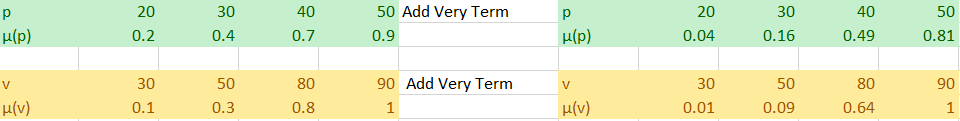
\includegraphics[scale=0.5]{pic_1}
	\end{figure}
	سپس از این دو تابع عضویت استفاده می‌کنیم تا رابطه \lr{R(v,p)} را پیاده‌سازی کنیم. ستون‌های \lr{p} و \lr{v} در تصویر مشخص شده است.
	\begin{figure}[H]
		\centering
		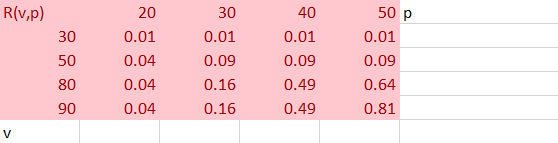
\includegraphics[scale=0.5]{pic_2}
	\end{figure}
	حال با توجه به اینکه ورودی ما بصورت \textbf{حجم تقریبا کم نباشد} است، ما ترم \textbf{کم} را به ترم \textbf{تقریبا کم نبودن} بصورت زیر تبدیل می‌کنیم.
	\begin{equation}
		\mu_{not\ fairly\ less} = 1 - (\mu_{less})^{\frac{1}{2}}
	\end{equation}
	\begin{figure}[H]
		\centering
		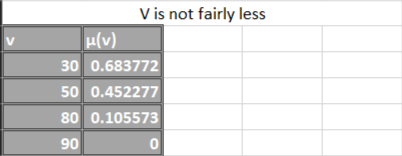
\includegraphics[scale=0.8]{pic_3}
	\end{figure}
	حال ورودی را به تابع \lr{R(v,p)} داده و خروجی می‌گیریم.
	\begin{figure}[H]
		\centering
		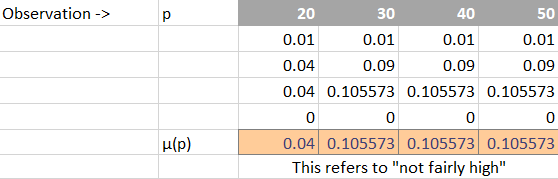
\includegraphics[scale=0.8]{pic_4}
	\end{figure}
	اعداد موجود در خط \lr{$\mu(p)$} همان خروجی تابع هستند.
	البته چون ورودی ما بصورت \textbf{حجم تقریبا کم نباشد} است، خروجی ما نیز بصورت \textbf{فشار تقریبا زیاد نباشد} می‌باشد زیرا توصیفگرها نیز به خروجی منتقل می‌شود. 
	\begin{equation}
		\mu_{high} = (1 - \mu_{not\ fairly\ high})^{2}
	\end{equation}
	\begin{figure}[H]
		\centering
		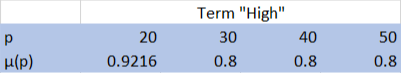
\includegraphics[scale=0.8]{pic_5}
	\end{figure}
	\section{سوال سوم}
		برای انجام محاسبات در این سوال، از \lr{Excel} استفاده شده است که فایل آن در همین پوشه موجود است.
	\newline
	برای پیدا کردن درستی هر یک از عبارات، ابتدا میزان درستی هر یک از مقدم‌ها را پیدا می‌کنیم. با توجه بکار رفتن لفظ \textbf{بسیار} در این عبارات، تابع عضویت این لفظ را  برای هر ترم \LTRfootnote{\lr{Term}} بصورت زیر تعریف می‌کنیم:
	\begin{equation}
		\mu_{very\ term} = (\mu_{term})^{2}
	\end{equation}
	سپس برای محاسبه اشتراک \LTRfootnote{\lr{AND}} بین ترم‌ها، از مینیمم استفاده می‌کنیم.
	
	\begin{equation}
		\mu_{term1\cap term2} = min(\mu_{term1}, \mu_{term2})
	\end{equation}
	سپس برای محاسبه رابطه شرطی \LTRfootnote{\lr{Implication}} بین دو ترم از رابطه زیر استفاده می‌کنیم:
	\begin{equation}
		v(A) \implies v(B) ::= max(1-v(A), v(B))
	\end{equation}
	\begin{figure}[H]
		\centering
		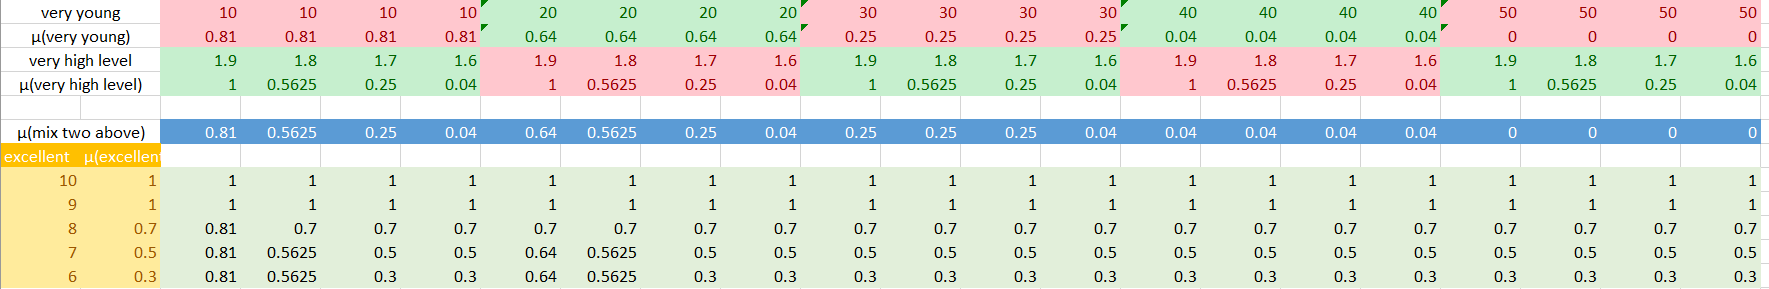
\includegraphics[scale=0.35]{pic_6}
		\caption{جدول میزان درستی‌های مربوط به گزاره اول}
		\label{t1}
	\end{figure}
	در جدول \ref{t1}، ابتدا میزان درستی مقدم یا همان $\mu_{very\ young\cap very\ high\ level}$ را پیدا می‌کنیم که حاصل آن همان $\mu_{mix\ two\ above}$ در جدول است. سپس با توجه به فرمول رابطه شرطی، میزان درستی گزاره خواسته شده را در بخش آبی جدول \ref{t1} پیدا می‌کنیم.
	\begin{figure}[H]
		\centering
		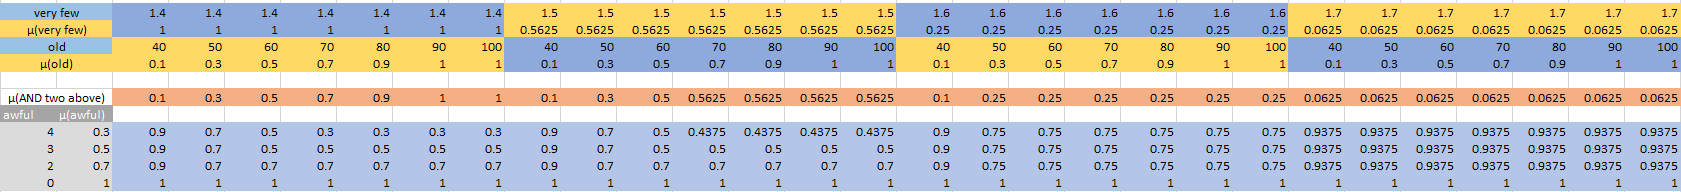
\includegraphics[scale=0.35]{pic_7}
		\caption{جدول میزان درستی‌های مربوط به گزاره دوم}
		\label{t2}
	\end{figure}
	برای جدول \ref{t2} نیز مشابه حدول قبلی، ابتدا حاصل $\mu_{very\ few\cap old}$ را پیدا کرده و سپس میزان درستی گزاره خواسته شده را می‌یابیم.
\end{document}
